\textbf{$\ket{\psi^-}=\frac{1}{\sqrt{2}} (\ket{01}-\ket{10})$} \vspace{.3cm}

\begin{quote}
    \begin{minted}[fontsize=\small, linenos, frame=single]{python}
estado_inicial = [0,1]
circuito_bell4 = QuantumCircuit(2)
circuito_bell4.initialize(estado_inicial,0)
circuito_bell4.initialize(estado_inicial,1)
circuito_bell4.h(0)
circuito_bell4.cx(0,1)                #cx: controlled x
circuito_bell4.measure_all()
circuito_bell4.draw('mpl')
    \end{minted}
    \vspace{.3cm}
    \begin{center}
        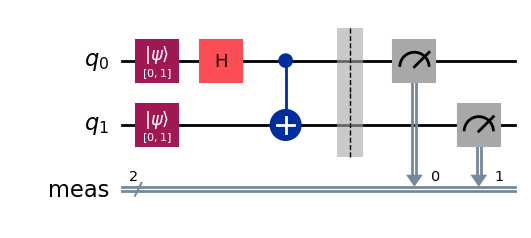
\includegraphics[height=3.3cm]{src/Img/3.3.png}
    \end{center}

    En este caso, usamos la combinación inicial $\ket{11}$:

    \begin{align*}
        \hat{C_x}\hat{H}\ket{11}
        = \hat{C_x} \left( \frac{1}{\sqrt{2}} (\ket{01}-\ket{11}) \right)
        = \frac{1}{\sqrt{2}} (\ket{01}-\ket{10})
    \end{align*}

    Podemos comprobar sacando el statevector, recordando que la base es $00,01,10,00$.
    \vspace{.5cm}

    \begin{center}
        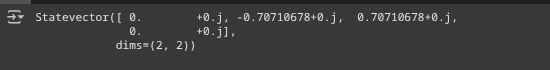
\includegraphics[width=.8\textwidth]{src/Img/3.3.r.png}
    \end{center}

    Algo raro en esta parte es que al sacar el statevector se le aplica una fase global pero
    no es algo importante para esto y el circuito es correcto.
\end{quote}
\vspace{.3cm}


\textbf{¿Cuál es la importancia de los estados de Bell en el cómputo cuántico?}\vspace{.3cm}

Son los primeros 4 estados en donde podemos ver \texttt{qubits} con comportamiento
entrelazado y superposición en donde, al medir uno el estado de ambos colapsa. De manera aplicada
lo podemos pensar como la manera en la que los qubits se comunican y dependen entre si unos de
otros.
